\section{System Evaluation}\label{seceval}
Reflecting on the objectives discussed in \textit{\ref{objectives}: Project Objectives}, the following is a condensed initial list of objectives for both the dissertation and applied aspects this project:\\

\textit{\textbf{Dissertation Objectives:}}
\begin{enumerate}
    \item Introduce the concept of the project.
    \item Provide the reader with a rounded understanding of cryptocurrencies.
    \item Explain to the reader how volatile cryptocurrency prices can be.
    \item Describe in detail the applied aspect of this project.
\end{enumerate}

\textit{\textbf{Applied Project Objectives:}}
\begin{enumerate}
    \item Create a simple web application which is easy to use and clear to understand.
    \item Deliver cryptocurrency prices to the user.
    \item Provide an educated guess as to future changes in prices.
    \item Work closely with the given learning outcomes for this project.
    \item Conduct work as a team, in a professional manner akin to what is expected in industry.
\end{enumerate}

\subsection{Testing}
Based on the objectives outlined above, the following tests were carried out to gain an insight as to the success and robustness of this application.

\subsubsection{Usability Testing}
Undoubtedly, a large portion of this project as whole surrounds explaining to the reader the fundamentals of cryptocurrency. The goals which cannot be quantified were considered to be all \textit{Dissertation Objectives}, and \textit{Objective 1} in the \textit{Applied Project Objectives} list. In order to measure the success of these goals, it was decided that the best was to do so was to ask others with varying levels of knowledge to read one or many chapters and briefly use the web application, and to gather feedback from them.

We created a survey through Google Forms, and sent its \textcolor{NavyBlue}{\href{https://docs.google.com/forms/d/e/1FAIpQLSfZQVFLgzG6dHy9U46xHPHuvzhitVnsvZaT1FXDjL-pFlgQTg/viewform?usp=sf_link}{link}} to those who had kindly offered to read this dissertation. All information other than the number of chapters read was on a scale of one to five.

The form asked participants five questions; their initial level of knowledge of cryptocurrency, which dissertation chapters they had read, how easy they felt terminology was to understand, how much the reading had improved their knowledge of cryptocurrencies, and how easy they felt the corresponding web application was to use. Identity remained anonymous, as it was deemed not required for the purpose of the survey. The link was only sent to those who had agreed to participate, and thus the form's results would not be skewed by anyone who had not participated.

A summary of the results is detailed in \textit{Figure \ref{surres}} below.

\begin{figure}[h]
    \centering
    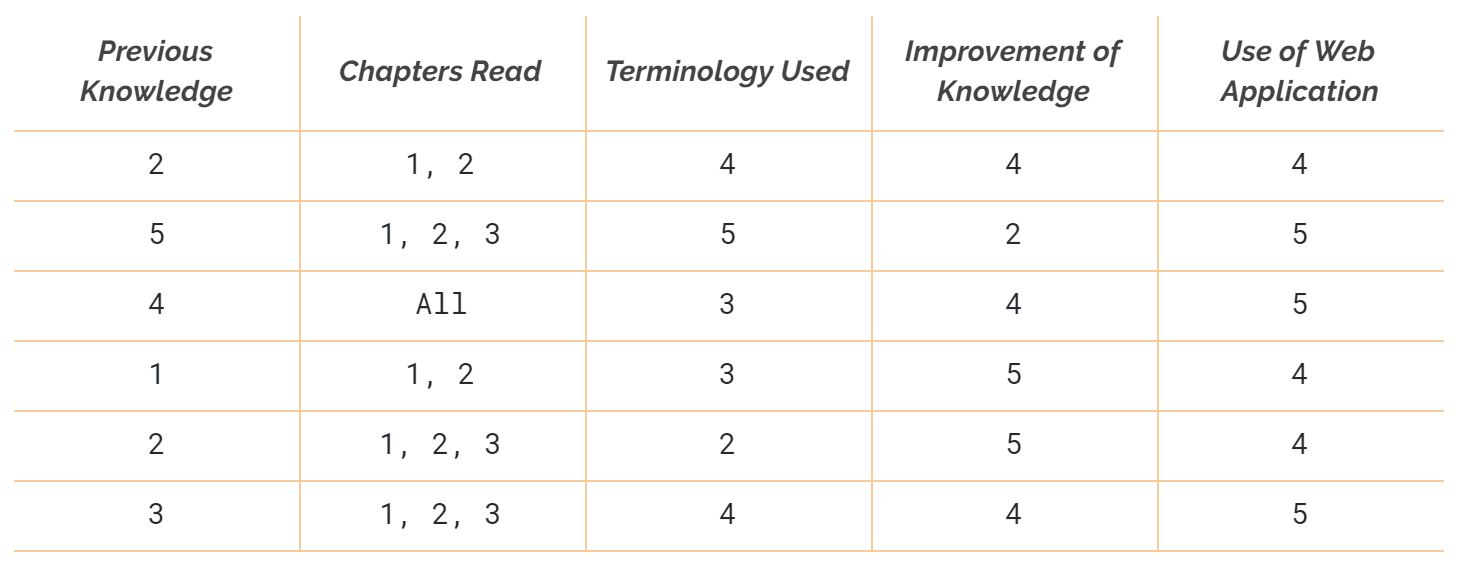
\includegraphics[width=0.9\textwidth, keepaspectratio]{img/testres.JPG}
    \caption{Survey Results \textit{April 2018}}
    \label{surres}
\end{figure}

Based on these results, we can conclude that while those with expert levels of initial knowledge did not learn much more, those with moderate or beginner levels of knowledge did increase that level of knowledge. For example, the second last entry details someone with initial knowledge of \textit{2} and following their reading of all three theoretical chapters, had felt their knowledge of the area had improved substantially.

\subsection{Evaluation of Objectives}
Following the objectives discussed above, the remaining objectives of the applied project were evaluated in the following ways: 

\textit{\textbf{Objective 2 - Deliver cryptocurrency prices to the user:}} Cryptocurrency prices were delivered to the user in the form of Bitcoin price in Euros, plotted on a graph contained in the web application home page. The data is obtained using the \mintinline{python}{forex-python} library, which is queried every thirty seconds for the latest Bitcoin price. The graph is updated to include this new value, with graph polling of data occurring every three seconds. This ensures that the prices are as up to date as can be.

\textit{\textbf{Objective 3 - Provide an educated guess as to future changes in prices:}} Through the use of machine learning, estimating the following day's closing price of Bitcoin has been achieved and implemented within the application. Due to the limitations of the system's prediction model, the estimate of close price is only applicable on a day to day basis and cannot be used for long term predictions, thus the system is retrained once per day on updated currency data. The predictions are delivered to the user via a graph, displaying previous predictions versus actual close prices. Unfortunately, natural language processing techniques were not implemented in this project, offering opportunity for future development.

\textit{\textbf{Objective 4 - Work closely with the given learning outcomes for this project:}} The expected learning outcomes for this project included applying appropriate research and development methodologies, demonstrating awareness of innovative technologies and incorporating them into the project where relevant, and the ability to critically evaluate the work and any potential for future work. As outlined in \textit{\ref{prelim}: Preliminary Research and Project Commencement}, the team conducted extensive research into a variety of different technologies and methodologies before beginning the project. While most of the project relies on faithful technologies such as Python, an effort was made to integrate newer technologies such as TensorFlow for Machine Learning, where it was deemed important to take advantage of the newest innovations in the field. Finally, the project has 

\textit{\textbf{Objective 5 - Conduct work as a team, in a professional manner akin to what is expected in industry:}} As discussed in \textit{\ref{issuesencountered}: Issues Encountered During the Development Process}, there were a number of problems faced by the team throughout this project's life cycle. All disagreements were discussed in a calm manner, giving each team member an equal platform on which to discuss their concerns. The team believe to have conducted themselves in a professional manner throughout the project, evident in the endurance of their friendships through any disagreements. 
\subsection{Opportunities for Improvement}
While the project achieved its initial objectives in some capacity or another, the point at which any project is complete and unable to be improved upon is difficult to pinpoint.

The preliminary planning of this project inevitably meant most of the technologies chosen were chosen for the right reasons, and if not were quickly replaced by more appropriate technologies. While the team is content with the technologies implemented in the final solution, there is of course opportunity for improvement with regard to extra features in the web application. 

\textit{\textbf{Wider Variety of Cryptocurrencies:}} Of course, it would be ideal to have all the major cryptocurrencies such as Ethereum, Litecoin, Ripple and the recently developed Bitcoin Cash implemented in and being predicted by this application. Due to time constraints and memory constraints with Heroku, it was deemed suitable to focus our efforts on the cryptocurrency with the largest market capitalisation; Bitcoin \cite{coinmarketcap}.

\textit{\textbf{Natural Language Processing:}} As mentioned in the initial \textit{\ref{objectives}: Objectives}, natural language processing can and has previously been used \cite{socmedimpact} to determine fluctuations in prices of cryptocurrency. This project could greatly benefit from such technology, through implementing a component which would search given sites for negative or positive discussions on cryptocurrencies. This information could be used to predict an incoming change of price, or simply display the changing popularity of given cryptocurrencies from day to day.

\textit{\textbf{Long Term Predictions:}} In addition to natural language processing, a neural network model for long-term prediction could also be implemented. Unfortunately the current application only estimates short-term values effectively, and the addition of a long-term estimate using both machine learning and natural language processing would make this application more attractive to those considering long-term investment in cryptocurrency.

\textit{\textbf{Docker:}} As outlined in \textit{\ref{secresearchmeth}: Research Methodology}, Docker was initially considered for its containerisation capabilities. The technology was not crucial and due to time constraints was not implemented to facilitate more crucial work being completed. However, the use of Docker in the system would add an extra layer of robustness, allowing for easy local deployment should the Heroku deployment ever be unavailable.

\subsection{Overall Evaluation}
To conclude, this application and dissertation have achieved the main objectives described in \textit{\ref{objectives}: Objectives} in full or some capacity. Based on usability tests, any given is likely to benefit from either the web application or the dissertation, or both. The project is built on solid and enduring technologies such as Python, with newer, innovative technologies such as TensorFlow incorporated to add an extra layer of interest and allure to the project. Despite numerous problems and associated delays, the project has achieved initial goals and objectives in an appropriate manner, leaving room for further additional development.